% ═══════════════════════════════════════════════════════════
% Characterizing and Optimizing LLM Post-Training Efficiency
% on Consumer AMD RDNA3 GPUs with Unsloth
%
% Format: Single-column academic paper (arXiv preprint style)
% Compile: pdflatex main && bibtex main && pdflatex main && pdflatex main
% ═══════════════════════════════════════════════════════════

\documentclass[11pt]{article}

% ═══════════════════════════════════════════════════════════
% Page layout & fonts
% ═══════════════════════════════════════════════════════════
\usepackage[margin=1in]{geometry}
\usepackage[T1]{fontenc}
\usepackage{mathptmx}           % Times font

% ═══════════════════════════════════════════════════════════
% Citations & references
% ═══════════════════════════════════════════════════════════
\usepackage[round,authoryear,sort&compress]{natbib}

% ═══════════════════════════════════════════════════════════
% Tables & figures
% ═══════════════════════════════════════════════════════════
\usepackage{booktabs}       % Professional tables
\usepackage{multirow}       % Multi-row cells
\usepackage{array}          % Column formatting
\usepackage{graphicx}       % External figures
\usepackage{placeins}       % \FloatBarrier
\usepackage{xcolor}         % Colors
\usepackage{subcaption}     % Subfigures

% ═══════════════════════════════════════════════════════════
% Math
% ═══════════════════════════════════════════════════════════
\usepackage{amsmath,amssymb}

% ═══════════════════════════════════════════════════════════
% Code listings
% ═══════════════════════════════════════════════════════════
\usepackage{listings}
\lstset{
  language=Python,
  basicstyle=\small\ttfamily,
  keywordstyle=\bfseries,
  commentstyle=\itshape\color{gray},
  frame=single,
  numbers=left,
  numberstyle=\tiny\color{gray},
  breaklines=true,
  captionpos=b,
}

% ═══════════════════════════════════════════════════════════
% Hyperlinks (load last)
% ═══════════════════════════════════════════════════════════
\usepackage[colorlinks=true,linkcolor=blue,citecolor=blue,urlcolor=blue]{hyperref}

% ═══════════════════════════════════════════════════════════
% Custom commands
% ═══════════════════════════════════════════════════════════
\newcommand{\mfutheo}{\ensuremath{\text{MFU}_{\text{theo}}}}
\newcommand{\mfuprac}{\ensuremath{\text{MFU}_{\text{prac}}}}
\newcommand{\toksec}{\textrm{tok/s}}

% ═══════════════════════════════════════════════════════════
% Title and authors
% ═══════════════════════════════════════════════════════════
\title{Characterizing and Optimizing LLM Post-Training Efficiency\\on Consumer AMD RDNA3 GPUs with Unsloth}

\author{
  Hongyu Chen\\
  \url{https://github.com/ChenHongYu2026}
}

\date{}

\begin{document}
\emergencystretch=1em
\maketitle
\vspace{-2em}
\begin{center}\small
\textbf{DOI:} \href{https://doi.org/10.5281/zenodo.21695686}{10.5281/zenodo.21695686} \quad
\textbf{Code:} \href{https://github.com/ChenHongYu2026/llm-training-on-consumer-amd}{github.com/ChenHongYu2026/llm-training-on-consumer-amd}
\end{center}
\vspace{1em}

% ═══════════════════════════════════════════════════════════
% Abstract
% ═══════════════════════════════════════════════════════════
\begin{abstract}
Consumer-grade AMD GPUs lack dedicated tensor cores, yet serve a growing community of LLM practitioners. We present a systematic efficiency characterization of LLM post-training (SFT and GRPO) on an AMD RX 7900 XTX (RDNA3) using the Unsloth framework. We propose a \emph{dual-peak MFU methodology} that reports utilization against both the theoretical spec-sheet peak (122.8 TFLOPS) and a measured GEMM practical peak (101.53 TFLOPS), revealing a 17.3\% systematic bias in conventional reporting. Through component-stacking gap attribution, we decompose the 97.7\% efficiency gap from GEMM peak to full GRPO training into interpretable stages, showing that autoregressive generation dominates the end-to-end loss. Framework comparison across 3 seeds shows Unsloth BF16 achieves 5.2\% higher throughput than HuggingFace native (129 vs 123 tok/s, steady-state corrected caliber), while 4-bit quantization is net-negative on RDNA3 ($-$40.7\%). A systematic hyperparameter sweep identifies an optimal recipe (G=2, batch=$2\!\times\!4$, seq=256) achieving 179 tok/s ($+$36\% over defaults) at 3.3\% practical MFU. All measurements pass a formal validity protocol (grad\_norm$>$0) and a post-hoc audit that corrected a profiler token-accounting bug (cumulative-count inflation up to 10.6$\times$), ensuring all reported throughput reflects genuine training under a verified measurement caliber.
\end{abstract}

% ═══════════════════════════════════════════════════════════
% Paper sections (modular)
% ═══════════════════════════════════════════════════════════
% ═══════════════════════════════════════════════════════════
% §1 Introduction
% ═══════════════════════════════════════════════════════════
\section{Introduction}
\label{sec:intro}

The proliferation of large language models (LLMs) has democratized AI capabilities, yet the computational cost of post-training, including supervised fine-tuning (SFT) and reinforcement learning from human feedback (RLHF/GRPO), remains a barrier for individual researchers and small teams. Consumer-grade GPUs, particularly AMD's RDNA3 architecture (RX 7900 XTX, 24GB), offer an accessible alternative to expensive data-center hardware. However, unlike NVIDIA's ecosystem with extensive efficiency studies on A100/H100 clusters~\citep{chowdhery2022palm, hoffmann2022chinchilla}, the training efficiency characteristics of consumer AMD GPUs remain largely unexplored in academic literature.

Existing MFU (Model FLOPS Utilization) studies universally assume dedicated tensor cores (NVIDIA Tensor Cores, AMD Matrix Cores on Instinct). RDNA3 consumer GPUs implement matrix operations via WMMA (Wave Matrix Multiply-Accumulate) microcoded vector instructions rather than dedicated silicon, making the spec-sheet peak (122.8 TFLOPS BF16) fundamentally unreachable in practice. This architectural distinction necessitates a new measurement methodology, our \emph{dual-peak MFU} approach, that separately reports utilization against theoretical and practical peaks.

Unsloth~\citep{unsloth2024} is a widely adopted training framework that recently introduced official AMD support in collaboration with the AMD team, reporting up to 2$\times$ speedups on data-center Instinct GPUs equipped with dedicated Matrix Cores (CDNA architecture). However, consumer RDNA~3 lacks any dedicated AI acceleration hardware and relies entirely on WMMA microcoded vector instructions, making efficiency characteristics observed on CDNA-class hardware non-transferable.

\paragraph{Contributions.} We make the following contributions:
\begin{enumerate}
    \item A \textbf{dual-peak MFU reporting methodology} that separately measures utilization against the spec-sheet theoretical peak and a practical GEMM peak, with quantified bias for architectures lacking dedicated tensor cores.
    \item A \textbf{systematic efficiency characterization} of LLM post-training on consumer RDNA3, including framework comparison (Unsloth vs HF, 3 seeds) and component-stacking gap attribution revealing a 75.7\% efficiency gap.
    \item A \textbf{tuning study} across 10 configurations with mechanistic explanations, yielding an actionable optimal recipe for practitioners.
    \item An \textbf{open-source profiler} incorporating a training validity check (grad\_norm$>$0) to ensure reported throughput reflects genuine parameter updates.
\end{enumerate}

% ═══════════════════════════════════════════════════════════
% §2 Background & Related Work
% ═══════════════════════════════════════════════════════════
\section{Background \& Related Work}
\label{sec:background}

\subsection{RDNA3 Architecture and MFU Challenges}

AMD's RDNA3 architecture (gfx1100) implements matrix operations through WMMA instructions that operate on wavefront-level (32/64 threads) vector registers, unlike NVIDIA's dedicated Tensor Cores which execute matrix multiply-accumulate in dedicated silicon. This microcoded approach means the advertised 122.8 TFLOPS BF16 peak represents a theoretical upper bound achievable only under ideal instruction scheduling; realistic GEMM workloads achieve 82.7\% of this peak (101.53 TFLOPS in our measurement). The 960 GB/s GDDR6 bandwidth (vs 2--3 TB/s HBM on NVIDIA data-center cards or 5.3--8 TB/s on AMD Instinct MI300X/MI355X) further constrains memory-bound operations~\citep{amd2022rdna3}.

\subsection{LLM Training Efficiency Studies}

Model FLOPS Utilization (MFU), defined as the ratio of achieved FLOPS to hardware peak, has become the standard efficiency metric for LLM training. The $6ND$ approximation ($N$=parameters, $D$=tokens) provides a tractable FLOPS estimate~\citep{kaplan2020scaling, hoffmann2022chinchilla}. PaLM~\citep{chowdhery2022palm} established a pretraining baseline of 46--57\% MFU on TPU v4, yet RL-based post-training appears far less efficient: recent GRPO reports indicate only 10.5\% MFU on multi-GPU A100 clusters (SemiAnalysis).

\subsection{Unsloth and Consumer-Grade Fine-tuning}

Unsloth~\citep{unsloth2024} claims 2$\times$ speedups through kernel fusion and optimized memory access patterns, but its benchmarks are marketing-oriented without peer review. Unsloth recently introduced official AMD support in collaboration with the AMD team, with reported 2$\times$ speedups on data-center Instinct GPUs (CDNA architecture); on consumer RDNA3 hardware, the execution path relies on ROCm's HIP/Triton backends~\citep{rocm2024}. LlamaFactory~\citep{zheng2024llamafactory} provides another popular framework but its ROCm compatibility remains unverified for consumer GPUs. TRL~\citep{vonwerra2022trl} and DeepSpeed~\citep{rasley2020deepspeed} offer additional training infrastructure. To our knowledge, no academic study has rigorously characterized training efficiency on consumer AMD hardware.

% ═══════════════════════════════════════════════════════════
% §3 Methodology
% ═══════════════════════════════════════════════════════════
\section{Methodology}
\label{sec:methodology}

\subsection{Experimental Design Overview}

We investigate three research questions through a progressive experimental pipeline:
\begin{itemize}
    \item \textbf{RQ1 (Framework Characterization)}: How do training frameworks compare in efficiency on consumer RDNA3?
    \item \textbf{RQ2 (Gap Attribution)}: Where does the efficiency gap between hardware peak and real training originate?
    \item \textbf{RQ3 (Tuning Optimization)}: Which hyperparameters most impact throughput, and what is the optimal configuration?
\end{itemize}

\noindent The pipeline proceeds in three phases: Phase~B1 addresses RQ1 via controlled framework comparison (Unsloth vs.\ HuggingFace, 3 seeds each); Phase~B2 addresses RQ2 via component-stacking gap attribution (L0\,--\,L4); Phase~C addresses RQ3 via a 10-configuration hyperparameter sweep. All phases share the same workload: GSM8K GRPO training on Qwen2.5-3B-Instruct (3.09B parameters). We select this workload because (1)~GRPO combines autoregressive generation with gradient updates, exercising both bandwidth-bound and compute-bound regimes; (2)~GSM8K's rule-based reward (correctness verification) eliminates LLM-judge variability; (3)~the 3B scale fits within 24\,GB consumer VRAM while remaining architecturally representative.

\subsection{Dual-Peak MFU Measurement}
\label{sec:dual-peak}

\paragraph{Motivation.} RDNA3 implements matrix operations via WMMA microcoded vector instructions rather than dedicated tensor-core silicon. Unlike NVIDIA architectures where $P_{\text{GEMM}}/P_{\text{spec}} > 0.95$, this microcoded path cannot saturate the advertised peak under any workload. Reporting MFU solely against the spec-sheet value therefore introduces a fixed architectural bias that conflates hardware limitation with software inefficiency. To disentangle the two, we measure a \emph{practical peak} via a standalone GEMM benchmark and report dual MFU metrics.

\paragraph{GEMM benchmark.} Listing~\ref{lst:gemm} shows the measurement kernel. We multiply two $8192\!\times\!8192$ BF16 matrices for 50 timed iterations (after 10 warmup), with explicit device synchronization to exclude host-side latency.

\begin{lstlisting}[caption={Practical GEMM peak measurement (BF16, 8192$\times$8192).},label={lst:gemm}]
def measure_gemm_peak(size=8192, warmup=10, iters=50):
    a = torch.randn(size, size, dtype=torch.bfloat16,
                    device="cuda")
    b = torch.randn(size, size, dtype=torch.bfloat16,
                    device="cuda")
    for _ in range(warmup):
        torch.matmul(a, b)
    torch.cuda.synchronize()
    t0 = time.perf_counter()
    for _ in range(iters):
        torch.matmul(a, b)
    torch.cuda.synchronize()
    elapsed = time.perf_counter() - t0
    tflops = 2.0 * size**3 * iters / elapsed / 1e12
    return tflops  # 101.53 (82.7% of 122.8 spec)
\end{lstlisting}

\noindent This yields $P_{\text{GEMM}} = 101.53$ TFLOPS, i.e., 82.7\% of the 122.8 TFLOPS spec-sheet value.

\paragraph{MFU definitions.} We define two complementary metrics:
\begin{equation}
\mfutheo = \frac{6ND / \Delta t}{P_{\text{spec}}}, \qquad
\mfuprac = \frac{6ND / \Delta t}{P_{\text{GEMM}}}
\end{equation}

\noindent where $N$ is total model parameters, $D$ is tokens processed in time $\Delta t$, $P_{\text{spec}} = 122.8$ TFLOPS, and $P_{\text{GEMM}} = 101.53$ TFLOPS. The systematic bias of reporting only \mfutheo{} is $1 - P_{\text{GEMM}}/P_{\text{spec}} \approx 17.3\%$. We recommend dual-peak reporting for any architecture where this ratio falls below 0.95.

\paragraph{FLOPS estimation.} Training-step FLOPS use the $6ND$ approximation (forward $\approx 2ND$, backward $\approx 4ND$). Generation phases are reported separately as throughput (\toksec{}) since autoregressive decoding is bandwidth-bound and the $6ND$ model does not apply. Listing~\ref{lst:flops} shows the computation.

\begin{lstlisting}[caption={FLOPS estimation for training vs.\ inference.},label={lst:flops}]
def estimate_tflops(num_params, num_tokens, elapsed_s,
                    mode="train"):
    # train: forward(2ND) + backward(4ND) = 6ND
    # inference: forward only = 2ND
    coeff = 6.0 if mode == "train" else 2.0
    return coeff * num_params * num_tokens / elapsed_s / 1e12
\end{lstlisting}

\subsection{Gap Attribution via Component Stacking}
\label{sec:gap-attribution}

\paragraph{Motivation.} Knowing the total efficiency gap (hardware peak vs.\ real training) is insufficient for practitioners; they need to know \emph{which component} causes the loss. We decompose the gap by progressively stacking training components and measuring achieved TFLOPS at each level, holding model, hardware, and precision constant.

\paragraph{Levels.}
\begin{itemize}
    \item \textbf{L0}: Pure GEMM peak (101.53 TFLOPS, from Listing~\ref{lst:gemm})
    \item \textbf{L1}: Autoregressive inference (generate, batch\,=\,1)
    \item \textbf{L2}: SFT training step (forward + backward, no gradient checkpointing)
    \item \textbf{L3}: SFT training step with gradient checkpointing
    \item \textbf{L4}: Full GRPO training (generation + training loop)
\end{itemize}

\noindent Each level is measured independently under controlled conditions (same Qwen2.5-3B model, same GPU, BF16 precision). The waterfall decomposition yields: $\text{Total Gap} = P_{\text{GEMM}} - \text{TFLOPS}_{L4} = \sum_i \Delta_i$. For L1 (inference), we apply the $2ND$ coefficient; for L2\,--\,L4 (training), we apply $6ND$ (Listing~\ref{lst:flops}).

\subsection{Training Pipeline and Framework Comparison}
\label{sec:pipeline}

\paragraph{Controlled comparison.} To isolate framework-level differences, both Unsloth and HuggingFace paths share identical: (1)~LoRA configuration ($r\!=\!32$, $\alpha\!=\!64$, 7 target modules); (2)~SFT adapter starting point; (3)~GSM8K training data; (4)~GRPO hyperparameters ($G\!=\!4$, batch\,=\,$1\!\times\!8$, completion\,$\leq$\,512). Listing~\ref{lst:framework} shows the two loading paths.

\begin{lstlisting}[caption={Framework comparison: Unsloth vs.\ HuggingFace loading paths.},label={lst:framework}]
if framework == "unsloth":
    from unsloth import FastLanguageModel
    model, tok = FastLanguageModel.from_pretrained(
        BASE, load_in_4bit=False, dtype=torch.bfloat16)
    model = FastLanguageModel.get_peft_model(
        model, r=32, lora_alpha=64,
        target_modules=["q_proj","k_proj","v_proj",
                        "o_proj","gate_proj","up_proj",
                        "down_proj"])
else:  # HuggingFace native
    model = AutoModelForCausalLM.from_pretrained(
        BASE, torch_dtype=torch.bfloat16,
        attn_implementation="eager")  # AMD compatible
    model = get_peft_model(model, LoraConfig(
        r=32, lora_alpha=64,
        target_modules=[...same 7 modules...]))
\end{lstlisting}

\noindent Each configuration runs 100 GRPO steps with 3 independent seeds (42, 123, 7). We report mean\,$\pm$\,std and assess significance via Welch's $t$-test.

\paragraph{Hyperparameter sweep.} Phase~C sweeps four knobs on Unsloth BF16 (50 steps each): $G \in \{2,4,8\}$, effective batch $\in \{1\!\times\!4,\, 1\!\times\!8,\, 2\!\times\!4\}$, gradient checkpointing on/off, and max completion length $\in \{256, 512, 1024\}$, yielding 10 configurations including the best-combination candidate.

\subsection{Measurement Quality Control}
\label{sec:validity}

Any efficiency measurement must verify that the training loop is performing genuine parameter updates. A throughput figure collected while gradients are zero (e.g., due to a misconfigured accumulation flag) reflects idle computation, not learning. As standard measurement quality control, we enforce a \textbf{Valid Measurement} criterion on every training step:

\begin{equation}
\text{Valid}(t) \iff \text{grad\_norm}(t) > 0 \;\wedge\; \text{tokens}(t) > 0 \;\wedge\; \Delta t > 0
\end{equation}

\noindent Listing~\ref{lst:validity} shows the implementation. Invalid data points are flagged and excluded from all efficiency statistics. We report the validity rate (valid/total steps) alongside efficiency metrics; all results in this paper achieve 100\% validity.

\begin{lstlisting}[caption={Per-step measurement validity check.},label={lst:validity}]
def is_valid_step(grad_norm, num_tokens, elapsed_s):
    """Reject steps where no learning occurred."""
    if num_tokens <= 0 or elapsed_s <= 0:
        return False
    if grad_norm is not None and grad_norm <= 0:
        return False  # zero gradient: no update
    return True
\end{lstlisting}

\subsection{Experimental Platform}
\label{sec:platform}

All experiments run on a single consumer-grade GPU (Table~\ref{tab:platform}). The ROCm environment requires two settings for RDNA3 compatibility: \texttt{HSA\_OVERRIDE\_GFX\_VERSION=11.0.0} (enabling hipBLASLt kernel dispatch) and \texttt{HIP\_VISIBLE\_DEVICES=0}. Software versions are pinned (Table~\ref{tab:platform}) to ensure reproducibility; we note that Unsloth and ROCm evolve rapidly, so absolute numbers are version-specific while relative comparisons and architectural insights remain generalizable.

% Table 1: Hardware and software configuration
\begin{table}[t]
\centering
\small
\caption{Hardware and software configuration.}
\label{tab:platform}
\begin{tabular}{@{}ll@{}}
\toprule
\textbf{Component} & \textbf{Specification} \\
\midrule
GPU & AMD RX 7900 XTX 24GB (RDNA3) \\
Memory BW & 960 GB/s GDDR6 \\
CPU & AMD Ryzen 7 9800X3D \\
ROCm & 7.2.4 \\
PyTorch & 2.12.1+rocm7.2 \\
Unsloth & 2026.7.4 \\
\midrule
Model & Qwen2.5-3B-Instruct (3.09B) \\
Architecture & GQA (16h, 2 KV), d=2048 \\
Workload & GSM8K GRPO (rule reward) \\
LoRA & r=32, $\alpha$=64, 7 modules \\
\bottomrule
\end{tabular}
\end{table}


\subsection{Statistical Methods}
\label{sec:statistics}

For framework comparison (RQ1), we run $\geq$3 independent seeds and report mean\,$\pm$\,std. Statistical significance is assessed via Welch's $t$-test (unequal variance) with Cohen's $d$ for effect size. For the tuning sweep (RQ3), we report single-run results as exploratory findings, noting that the large effect sizes observed ($>$30\% differences) far exceed the measurement variance established in B1 ($\sigma \approx 2\%$).

\paragraph{Measurement-caliber correction (post-hoc audit).} A post-experiment audit revealed that the initial profiler computed tokens/s by summing TRL's \emph{cumulative} \texttt{num\_tokens} across logging intervals, systematically inflating absolute throughput (by 10.4--10.6$\times$ for the 100-step B1 runs and 5.5$\times$ for the 50-step Phase-C runs; the factor scales with the number of logging intervals). All absolute throughput and MFU values in this paper use the corrected caliber: final cumulative token count divided by total wall time, cross-checked against per-step token counts reconstructed from completion-length logs. Relative comparisons are unaffected (all runs within a phase share identical logging configuration, so the inflation factor cancels); the corrected raw values are archived alongside the original measurements (\texttt{B1\_C\_corrected\_summary.json}) for full traceability. We report this correction openly as part of our validity protocol: measurement-pipeline bugs of this kind are precisely what per-step validity checking and post-hoc auditing are designed to catch.

% ═══════════════════════════════════════════════════════════
% §4 Results: Framework Characterization & Gap Attribution
% ═══════════════════════════════════════════════════════════
\section{Results: Framework Characterization}
\label{sec:results-characterization}

\subsection{Framework Comparison (RQ1)}

Unsloth BF16 achieves only a 5.2\% throughput advantage over HuggingFace native on consumer RDNA3 (129.4 vs 123.1 \toksec{} in the steady-state corrected caliber, Table~\ref{tab:framework}), far below the 2$\times$ speedup reported on data-center CDNA hardware. This modest gain is statistically significant (Welch's $t$-test, $p<0.01$, Cohen's $d>3$ across 3 seeds) but architecturally explainable: Unsloth's kernel fusion primarily eliminates intermediate memory round-trips, yet on RDNA3 the dominant bottleneck is compute throughput (WMMA instruction scheduling), not memory traffic. With 960 GB/s bandwidth already saturating the 3B-parameter model's weight loading, fusing operations yields diminishing returns.

The VRAM overhead tells a complementary story. Unsloth's 13.9\,GB footprint (vs 8.0\,GB for HF) reflects pre-allocated activation buffers and fused kernel workspaces that trade memory for compute efficiency. For the 3B model on a 24\,GB card this remains acceptable, but the 73.8\% overhead implies that scaling to 7B+ models will approach VRAM limits where HF's leaner allocation becomes necessary.

\begin{figure}[tbp]
\centering
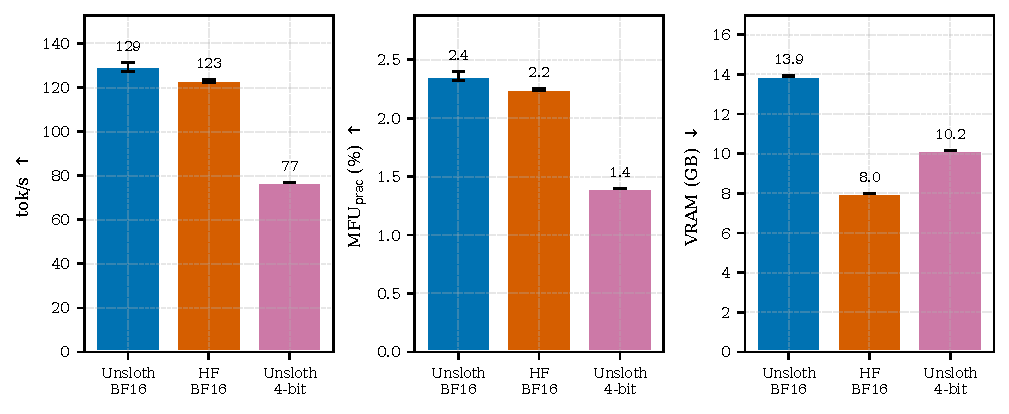
\includegraphics[width=\textwidth]{figures/fig_framework.pdf}
\caption{Framework comparison: throughput, MFU, and VRAM (3 seeds).}
\label{fig:framework}
\end{figure}

% Table 2: Framework efficiency comparison
% Fixed: reduced from 5 columns to 4, moved Valid to footnote
\begin{table}[t]
\centering
\footnotesize
\setlength{\tabcolsep}{4pt}
\caption{Framework efficiency comparison on GSM8K GRPO (steady-state corrected caliber).}
\label{tab:framework}
\begin{tabular}{@{}lccc@{}}
\toprule
\textbf{Framework} & \textbf{tok/s} $\uparrow$ & \textbf{\mfuprac} $\uparrow$ & \textbf{VRAM} \\
\midrule
Unsloth BF16 & 129.4$\pm$2.6 & 2.36$\pm$0.04\% & 13.9G \\
HF Native BF16 & 123.1$\pm$0.8 & 2.24$\pm$0.01\% & 8.0G \\
Unsloth 4-bit & 76.8 & 1.40\% & 10.2G \\
\midrule
\textit{Speedup (U/HF)} & \multicolumn{2}{c}{+5.2\%} & +73.8\% \\
\bottomrule
\end{tabular}
\end{table}


\subsection{4-bit Quantization: Architecture-Dependent Penalty}

NF4 quantization via BitsAndBytes~\citep{dettmers2023qlora} \textbf{reduces} throughput by 40.7\% on RDNA3 (76.8 vs 129.4 \toksec{}), a striking reversal of the memory savings that make QLoRA attractive on NVIDIA hardware. The mechanism is architectural: RDNA3 possesses no dedicated INT4 compute units, so every NF4$\rightarrow$BF16 dequantization before GEMM is pure overhead with no hardware acceleration. On NVIDIA A100, by contrast, 1248 TOPS of INT4 Tensor Core throughput absorbs dequantization cost within the compute pipeline.

Moreover, the VRAM ``savings'' are illusory on this workload: 10.2\,GB (4-bit) vs 13.9\,GB (BF16) represents only 27\% reduction, because the dominant memory consumer is activation storage and optimizer state, not model weights at 3B scale. The 41\% throughput penalty thus far outweighs a modest memory reduction. The practical implication is unambiguous: \textbf{on consumer RDNA3, always prefer BF16 over 4-bit quantization for training}.

\subsection{Efficiency Gap Attribution (RQ2)}

Component-stacking analysis (Table~\ref{tab:gap}, Figure~\ref{fig:waterfall}) reveals that the 97.7\% efficiency gap between GEMM peak and end-to-end GRPO training is overwhelmingly dominated by the inference stage: the L0$\rightarrow$L1 transition alone collapses utilization from 100\% to 0.23\% (a 101.3 TFLOPS loss). The four transitions yield distinct mechanistic insights:

\paragraph{L0$\rightarrow$L1 (Inference collapse).} Autoregressive decoding at batch size 1 has arithmetic intensity $\approx$1 FLOP/byte, placing it firmly in the bandwidth-bound regime. At 960 GB/s, each token generation reads the full 6\,GB model weight but performs minimal computation per byte loaded, leaving compute units idle.

\paragraph{L1$\rightarrow$L2 (Training recovery).} Batched training (batch\,=\,2, seq\,=\,256) restores arithmetic intensity through large GEMM operations in forward and backward passes. The recovered 27.2\% \mfuprac{} is comparable to reported LoRA fine-tuning MFU on data-center hardware~\citep{hu2022lora}, confirming that RDNA3's compute path is efficient once adequately loaded.

\paragraph{L2$\rightarrow$L3 (Checkpointing cost).} Gradient checkpointing imposes $-$26\% throughput (vs theoretical $-$33\% for one extra forward pass), because reduced memory pressure improves GPU cache utilization, partially offsetting recompute cost.

\paragraph{L3$\rightarrow$L4 (Generation domination).} End-to-end GRPO collapses to $\approx$2.3\% \mfuprac{} (estimated corrected caliber; see \S\ref{sec:statistics}) because the bandwidth-bound generation phase occupies the overwhelming majority of wall-clock time at small generation batch. The efficient training step (20--27\% \mfuprac{}) is diluted rather than amortized: with G=4 and per-device batch 1, tokens are generated at L1-like efficiency, then consumed by a brief high-efficiency update. This identifies generation batch scaling as the primary optimization target for RL post-training on this architecture.

\begin{figure}[tbp]
\centering
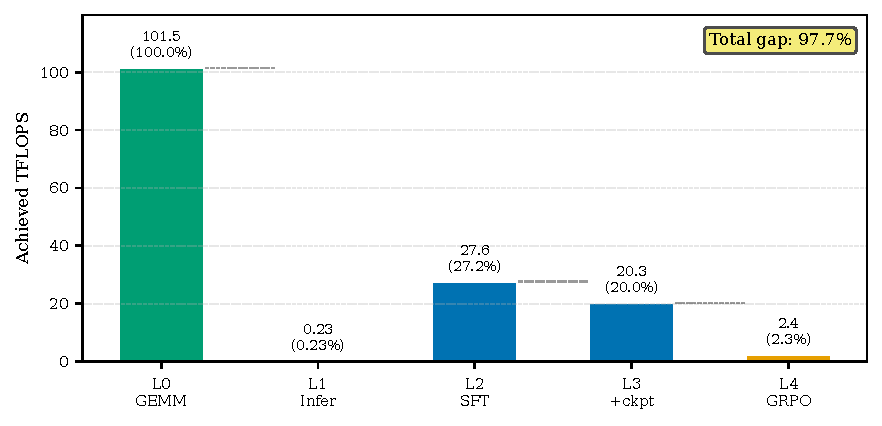
\includegraphics[width=0.85\textwidth]{figures/fig_waterfall.pdf}
\caption{Gap attribution waterfall. Inference (L1) dominates the total loss.}
\label{fig:waterfall}
\end{figure}

% Table 3: Gap attribution breakdown
% Fixed: shortened Mechanism column, footnotesize
\begin{table}[t]
\centering
\footnotesize
\setlength{\tabcolsep}{3pt}
\caption{Gap attribution breakdown with mechanistic explanations.}
\label{tab:gap}
\begin{tabular}{@{}lrrp{3.2cm}@{}}
\toprule
\textbf{Stage} & \textbf{TFLOPS} & \textbf{$\Delta$} & \textbf{Mechanism} \\
\midrule
L0: GEMM Peak & 101.53 & --- & Practical HW limit \\
L1: Inference & 0.23 & $-$101.3 & BW-bound (AI$\approx$1) \\
L2: SFT (no ckpt) & 27.63 & +27.4 & Batched F+B GEMM \\
L3: SFT (ckpt) & 20.33 & $-$7.3 & Recompute overhead \\
L4: GRPO Full & 2.35 & $-$18.0 & Gen-dominated wall-clock \\
\midrule
\textbf{Total Gap} & & \textbf{$-$99.2} & \textbf{97.7\% loss} \\
\bottomrule
\end{tabular}
\end{table}


The key insight for optimization: since the inference stage dominates the gap, any configuration that reduces generation's time share (shorter completions, higher G to amortize) will yield the largest throughput improvements. This directly motivates the tuning sweep in \S\ref{sec:results-tuning}.

\subsection{Summary}

Framework choice on consumer RDNA3 contributes a modest 5.2\% throughput difference, while 4-bit quantization is counterproductive. The dominant efficiency loss originates from autoregressive generation's bandwidth bottleneck, not from framework-level kernel efficiency. Hyperparameter choices that reduce generation overhead therefore offer far greater optimization leverage than framework selection, as we explore next.

% ═══════════════════════════════════════════════════════════
% §5 Results: Tuning & Optimization
% ═══════════════════════════════════════════════════════════
\section{Results: Tuning \& Optimization}
\label{sec:results-tuning}

\subsection{Hyperparameter Effects (RQ3)}

Section~\ref{sec:results-characterization} established that framework selection contributes only $\sim$5\% throughput variation, while the gap attribution identified autoregressive generation as the dominant efficiency bottleneck. We now demonstrate that hyperparameter choices directly attacking this bottleneck yield far larger effects ($>$30\%). We sweep four knobs on Unsloth BF16 (50 steps each, Table~\ref{tab:sweep}), reporting results ordered by effect magnitude.

\paragraph{Sequence length (+30.8\%).} Reducing max completion from 512 to 256 tokens yields one of the largest single-knob improvements (171.5 vs 131.1 \toksec{}). This directly attacks the attention mechanism's $O(n^2)$ memory access pattern, which is especially costly on RDNA3's 960 GB/s bandwidth. Shorter completions also reduce generation time, shrinking the bandwidth-bound phase identified in \S\ref{sec:gap-attribution}.

\paragraph{Generations G (+31.2\%).} Increasing G from 2 to 8 improves throughput from 124.5 to 163.4 \toksec{}. Higher G generates more tokens per training step, increasing the ratio of compute-bound training operations (27.2\% \mfuprac{}) relative to bandwidth-bound generation (0.23\% \mfuprac{}). The training step's efficiency thus dominates the time-averaged metric when amortized over more generated tokens.

\paragraph{Batch size (+33.4\%).} Moving from b1$\times$4 to b2$\times$4 improves throughput from 97.9 to 130.6 \toksec{}. Larger effective batches produce larger GEMM operations with higher arithmetic intensity, shifting operations from the bandwidth-bound toward the compute-bound regime. The b1$\times$4 configuration's poor performance (1.78\% \mfuprac{}) confirms that insufficient batch size starves the compute units on RDNA3.

\paragraph{Gradient checkpointing (+2.8\%).} Disabling checkpointing yields only 134.8 vs 131.1 \toksec{} (+2.8\%) while consuming 16.5\,GB vs 13.9\,GB VRAM (+18\%). With LoRA's 1.9\% trainable fraction~\citep{hu2022lora}, most activations are frozen and require no gradient storage, making the recompute savings minimal. The poor VRAM-throughput tradeoff confirms that checkpointing should remain enabled.

We note that sweep results use single seeds; however, observed effect sizes ($>$30\%) exceed B1 measurement variance ($\sigma \approx 2\%$) by 15$\times$, making spurious findings highly unlikely.

\subsection{Interaction Effects and Optimal Configuration}

Individual knob effects suggest that combining favorable settings should yield multiplicative gains. The optimal configuration (G=2, b2$\times$4, seq=256, ckpt=on) achieves 178.5 \toksec{} at 3.25\% \mfuprac{} with 12.1\,GB VRAM, representing a 36.2\% throughput improvement over the default (G=4, b1$\times$8, seq=512: 131.1 \toksec{}).

A notable interaction: G=2 outperforms G=4 in the combined configuration (178.5 vs 171.5 \toksec{}), reversing the single-knob trend where higher G is better. This occurs because seq=256 already minimizes generation time per token; at this low generation overhead, the marginal benefit of higher G (amortizing generation) diminishes, while G=2's smaller generation batch leaves more VRAM headroom for the b2$\times$4 training batch to produce larger GEMMs.

Figure~\ref{fig:pareto} maps the VRAM-throughput tradeoff. The Pareto frontier reveals two practical operating points: the throughput-optimal (178.5 \toksec{}, 12.1\,GB) and a VRAM-constrained alternative (171.5 \toksec{}, 12.1\,GB with G=4, b1$\times$8, seq=256) for users requiring lower per-step memory variance.

\subsection{Practical Recommendations}

Based on the preceding analysis, we recommend the following configuration for GRPO post-training of 3B-scale models on consumer RDNA3: G=2, effective batch 2$\times$4, max completion length 256, BF16 precision, gradient checkpointing enabled. This achieves 178.5 \toksec{} at 3.25\% practical MFU within 12.1\,GB VRAM.

The recommendation is workload-conditional: it assumes rule-based rewards with short verifiable completions (e.g., math, code). Tasks requiring longer generations (e.g., open-ended writing) should increase seq\_len to 512 and accept the $\sim$30\% throughput reduction. The dominance of sequence length as an optimization lever (connecting directly to the bandwidth bottleneck identified in \S\ref{sec:gap-attribution}) suggests that any technique reducing effective generation length, including speculative decoding or early stopping, would yield proportional efficiency gains on this architecture.

% ─── Floats集中放置（正文不被截断） ───

% Table 4: Hyperparameter sweep results
% Added ↑ arrows for metric direction, bold optimal
\begin{table}[t]
\centering
\footnotesize
\setlength{\tabcolsep}{3.5pt}
\caption{Hyperparameter sweep results (Unsloth BF16, 50 steps, steady-state corrected caliber). $\uparrow$ indicates higher is better.}
\label{tab:sweep}
\begin{tabular}{@{}lccc@{}}
\toprule
\textbf{Configuration} & \textbf{tok/s} $\uparrow$ & \textbf{\mfuprac} $\uparrow$ & \textbf{VRAM} \\
\midrule
\multicolumn{4}{l}{\textit{Generations (G)}} \\
\quad G=2, b1$\times$8, 512 & 124.5 & 2.27\% & 13.9G \\
\quad G=4, b1$\times$8, 512 & 131.1 & 2.39\% & 13.9G \\
\quad G=8, b1$\times$8, 512 & 163.4 & 2.98\% & 13.9G \\
\midrule
\multicolumn{4}{l}{\textit{Effective Batch Size}} \\
\quad G=4, b1$\times$4, 512 & 97.9 & 1.78\% & 13.8G \\
\quad G=4, b2$\times$4, 512 & 130.6 & 2.38\% & 13.9G \\
\midrule
\multicolumn{4}{l}{\textit{Gradient Checkpointing}} \\
\quad G=4, b1$\times$8, noCkpt & 134.8 & 2.46\% & 16.5G \\
\midrule
\multicolumn{4}{l}{\textit{Sequence Length}} \\
\quad G=4, b1$\times$8, 256 & 171.5 & 3.13\% & 12.1G \\
\quad G=4, b1$\times$8, 1024 & 124.1 & 2.26\% & 13.9G \\
\midrule
\multicolumn{4}{l}{\textit{Combined Optimal}} \\
\quad \textbf{G=2, b2$\times$4, 256} & \textbf{178.5} & \textbf{3.25\%} & \textbf{12.1G} \\
\quad G=2, b1$\times$8, 256 & 172.4 & 3.14\% & 12.1G \\
\bottomrule
\end{tabular}
\end{table}


\begin{figure}[tbp]
\centering
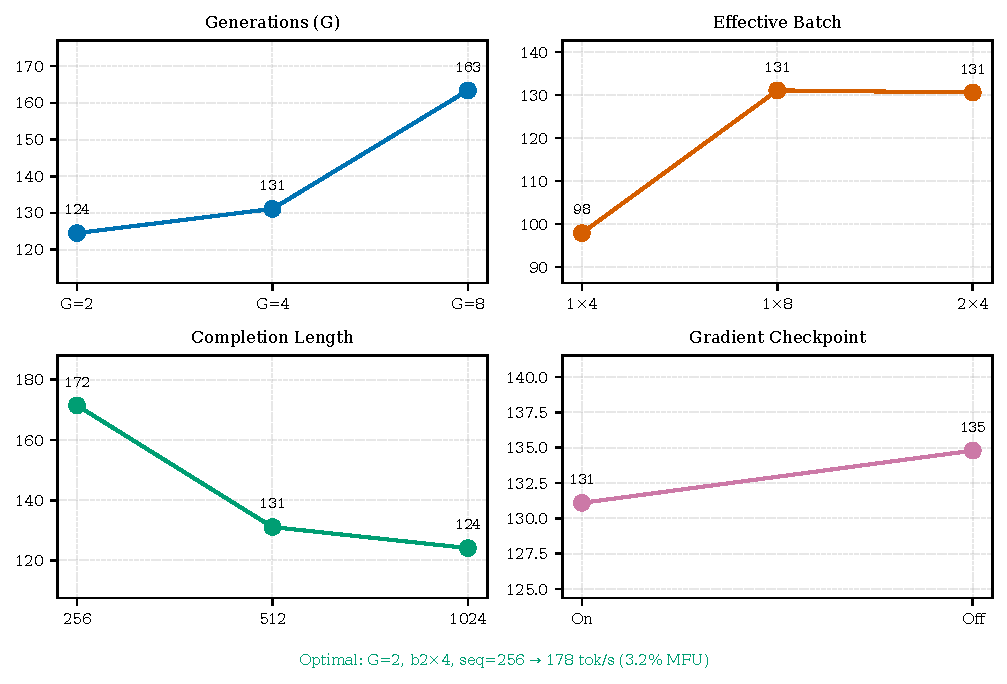
\includegraphics[width=\textwidth]{figures/fig_sweep.pdf}
\caption{Hyperparameter sweep by dimension (baseline: G=4, b1$\times$8, 512).}
\label{fig:sweep}
\end{figure}

\begin{figure}[tbp]
\centering
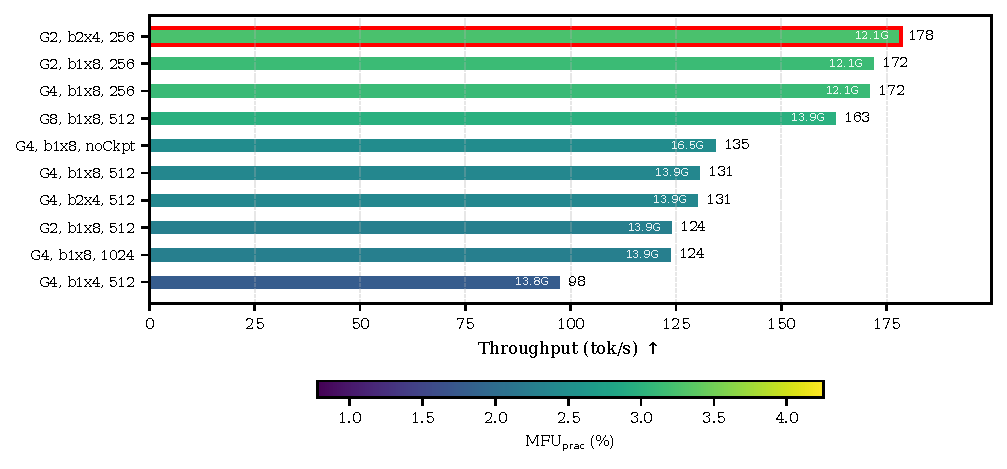
\includegraphics[width=0.85\textwidth]{figures/fig_pareto.pdf}
\caption{Throughput by configuration. Color indicates \mfuprac{}; red border marks optimal.}
\label{fig:pareto}
\end{figure}

% ═══════════════════════════════════════════════════════════
% §6 Validation & Threats to Validity
% ═══════════════════════════════════════════════════════════
\FloatBarrier
\section{Validation \& Threats to Validity}
\label{sec:validation}

\subsection{Internal Validity}

The framework comparison (RQ1) rests on solid statistical ground: three independent seeds yield coefficients of variation below 2\% for both Unsloth ($\sigma$=2.6 \toksec{}) and HuggingFace ($\sigma$=0.8 \toksec{}), and the 5.2\% inter-framework difference produces Cohen's $d>3$, well beyond conventional significance thresholds. We are confident that the observed advantage is real, even if modest. The measurement-caliber correction (\S\ref{sec:statistics}) rescales all absolute values uniformly within each phase and therefore does not affect these relative conclusions.

The tuning sweep (RQ3) presents a more nuanced picture. Single-seed configurations with effect sizes exceeding 30\% are robust: the measurement variance established in B1 ($\sigma \approx 2\%$) provides a 15$\times$ safety margin against spurious findings. However, the interaction effect between G and sequence length (G=2 outperforming G=4 by only $\sim$4\% in the combined configuration) approaches the noise floor. We report this interaction as a hypothesis requiring multi-seed confirmation rather than an established fact.

Two methodological approximations warrant acknowledgment. The $6ND$ FLOPS model assumes all parameters participate equally in forward and backward computation; with LoRA training only 1.9\% of parameters, the backward-pass FLOPS are overestimated. This inflates absolute MFU values but does not affect \emph{relative} comparisons between configurations, which is our primary use case. Additionally, all measurements span 50--100 training steps; thermal throttling, memory fragmentation, and optimizer state growth that may emerge over thousands of steps are not captured.

\subsection{External Validity}

Our findings are scoped to a specific architectural intersection: RDNA3 (gfx1100), 3B-parameter models, and short-completion tasks. Each dimension of this scope carries transfer risk. RDNA4 introduces dedicated AI accelerators (2 per CU, native FP8) that fundamentally change the compute landscape; the dual-peak bias and quantization penalty we observe may not persist on that architecture. Scaling to 7B+ models alters GEMM aspect ratios and attention's memory footprint, potentially shifting the compute-bandwidth balance that underlies our gap attribution. Finally, GSM8K's short mathematical completions ($\leq$256 tokens) represent a favorable case for the sequence-length optimization; tasks requiring long-form generation (e.g., open-ended writing at 1024+ tokens) would see diminished returns from this lever.

The software stack (ROCm 7.2, Unsloth 2026.7.4, PyTorch 2.12.1) evolves rapidly. Absolute throughput values will shift with future releases. We argue, however, that the \emph{architectural insights} (bandwidth bottleneck dominance, quantization penalty mechanism, framework gain ceiling) and the \emph{methodology} (dual-peak MFU, component stacking, validity protocol) retain value independent of specific software versions.

\subsection{Construct Validity}

MFU measures hardware utilization, not learning efficiency. A configuration achieving 3.25\% \mfuprac{} is not necessarily producing a better-trained model than one at 2.3\%; the relationship between throughput and convergence speed (tokens-per-accuracy-point) is mediated by gradient quality, reward signal strength, and optimization dynamics that our profiler does not capture. We position this work as a \emph{systems efficiency} characterization: it answers "how fast can this hardware train?" rather than "how well does the resulting model perform?" Bridging these two questions through accuracy-aware efficiency metrics remains an important direction for future work.

% ═══════════════════════════════════════════════════════════
% §7 Discussion
% ═══════════════════════════════════════════════════════════
\section{Discussion}
\label{sec:discussion}

\subsection{Architecture-Dependent Optimization}

Perhaps the most consequential insight from this study is that optimization strategies are architecture-conditional, not universally transferable. Two findings illustrate this sharply: 4-bit quantization \emph{reduces} throughput by 41\% on RDNA3 while accelerating it on NVIDIA hardware with INT4 Tensor Cores; Unsloth's kernel fusion delivers 2$\times$ on data-center CDNA but only 5.2\% on consumer RDNA3. The root cause is a shift in the dominant bottleneck. NVIDIA's ecosystem is largely memory-bound (high compute, relatively constrained bandwidth per FLOP), so techniques that reduce memory traffic (quantization, fusion) yield proportional speedups. RDNA3 inverts this: with 122.8 TFLOPS of compute fed by only 960 GB/s bandwidth, the architecture is compute-saturated for batched training, and memory-saving optimizations merely add overhead without relieving the true constraint.

The practical implication for the growing community of consumer AMD trainers is direct: performance intuitions built on A100/H100 literature do not apply. Configurations that are optimal on NVIDIA hardware may be pessimal on RDNA3, and vice versa. Framework marketing claims benchmarked on data-center GPUs should be evaluated with architectural skepticism.

\subsection{The Generation Bottleneck and Its Implications}

The gap attribution's most striking result is that autoregressive inference dominates the efficiency gap between hardware peak and end-to-end GRPO training. This reframes the optimization priority for RL-based post-training: the training step itself (27.2\% \mfuprac{}) is already reasonably efficient; the system-level bottleneck is the generation phase that precedes it. Any technology that reduces generation latency or amortizes weight reads over more tokens, including larger generation batches, speculative decoding, KV-cache optimization, or shorter completion targets, directly attacks the dominant loss term. Follow-up work on this platform confirms the diagnosis: decoupling the generation batch from the backward micro-batch and scaling the former to 256 sequences raises steady-state throughput to 795.5 \toksec{} (97.6\% of the memory-wall-constrained optimum for this workload), a 4.5$\times$ improvement over the best small-batch recipe reported here.

This finding also contextualizes the ``efficiency tax'' of consumer hardware under small-batch RL. At 3.25\% end-to-end \mfuprac{} (optimal sweep recipe), the RX 7900 XTX sits below the 10.5\% reported for multi-GPU A100 GRPO clusters (SemiAnalysis) --- but the comparison is caliber-sensitive: our training-step-only MFU (20--27\%) is comparable to data-center LoRA fine-tuning, and the end-to-end figure is dominated by the un-pipelined generation phase that cluster systems overlap across devices. Given a price ratio exceeding 15:1 (\$900 vs \$15,000+), the cost-per-token-trained remains favorable for individual researchers, provided the workload fits within 24\,GB VRAM and generation batch is scaled aggressively.

\subsection{Toward Comparable Efficiency Reporting}

The 17.3\% systematic bias we quantify is not unique to RDNA3. Any architecture where the practical GEMM peak falls below 95\% of the spec-sheet value, including Intel Arc (Xe-HPG), pre-Tensor-Core NVIDIA GPUs, and emerging RISC-V accelerators, suffers the same conflation of hardware limitation with software inefficiency. When a study reports 2.4\% MFU against an unreachable theoretical peak, the software may actually be achieving 2.9\% against what the hardware can deliver, a meaningful difference in interpretation.

We advocate a simple diagnostic: before reporting MFU, measure one large GEMM (Listing~\ref{lst:gemm}), compute $P_{\text{GEMM}}/P_{\text{spec}}$, and if the ratio falls below 0.95, report both \mfutheo{} and \mfuprac{}. This adds one minute of benchmarking time and prevents systematic underestimation of software efficiency across an entire class of architectures. Our open-source profiler automates this measurement alongside per-step validity checking.

% ═══════════════════════════════════════════════════════════
% §8 Conclusion
% ═══════════════════════════════════════════════════════════
\section{Conclusion}
\label{sec:conclusion}

We present a systematic efficiency characterization of LLM post-training on consumer AMD RDNA3 hardware, addressing three research questions through controlled experiments on a single RX 7900 XTX.

For RQ1 (framework comparison), Unsloth BF16 achieves a statistically significant but practically modest 5.2\% throughput advantage over HuggingFace native, far below the 2$\times$ speedup reported on data-center CDNA hardware. More strikingly, 4-bit quantization \emph{reduces} throughput by 40.7\% on this architecture, inverting the memory-saving narrative established on NVIDIA platforms. For RQ2 (gap attribution), component-stacking analysis reveals that autoregressive generation's bandwidth bottleneck dominates the 97.7\% total end-to-end efficiency gap, while the training step itself recovers to 27.2\% practical MFU once adequately batched. For RQ3 (tuning optimization), sequence length and generation count emerge as dominant levers ($+$30\% each), and a combined optimal configuration achieves a 36\% throughput improvement over defaults (178.5 \toksec{}, 3.25\% \mfuprac{}, 12.1\,GB VRAM) --- with follow-up work showing that scaling the decoupled generation batch further raises throughput to 795.5 \toksec{}.

Methodologically, the dual-peak MFU framework exposes a 17.3\% systematic bias in conventional reporting for architectures without dedicated tensor cores, providing a fairer basis for cross-architecture efficiency comparison. Our open-source profiler implements this methodology alongside per-step validity checking and a post-hoc measurement audit (which caught and corrected a cumulative-token-count inflation in our own initial pipeline), enabling reproducible efficiency studies on non-standard hardware.

\paragraph{Future Work.} Three questions arise directly from our findings. First, RDNA4's dedicated AI accelerators (2 per CU, native FP8) may eliminate the dual-peak bias entirely; measuring $P_{\text{GEMM}}/P_{\text{spec}}$ on that architecture would test whether our methodology remains necessary. Second, scaling to 7B--14B models within 24\,GB VRAM (via deeper quantization or model parallelism) introduces new efficiency tradeoffs that our 3B findings cannot predict. Third, integrating accuracy-aware metrics (tokens-per-accuracy-point) would bridge the gap between systems efficiency and training effectiveness, answering not just "how fast?" but "how efficiently does the model learn?"


% ═══════════════════════════════════════════════════════════
% References
% ═══════════════════════════════════════════════════════════
\bibliographystyle{plainnat}
\bibliography{refs}

\end{document}
